% This is the template for the writing report
% Figures and this .tex file should be put using relative path
% Figures are in the figures folder
% You only need to make changes of this .tex file and submit .pdf after converting this to .pdf
% Ignore other files in this folder
\documentclass{article}
\usepackage{float}
\usepackage{graphicx}
\usepackage{caption}
\usepackage{subcaption}
\usepackage{array}
\usepackage{geometry}
\usepackage{amsmath, bm}
\title{Machine Learning-Based Cryptocurrency Price Prediction} % come up with a good title
\author{Andrew Cooke, Yu Wang, Xinming Dai}
\geometry{left=3cm} 

\begin{document}
\maketitle
\begin{abstract}
Cryptocurrenies are not only used as a way of transaction. Major companies like Tesla starts to invest cryptos, and crypto even goes to war in Ukraine. The market sees high volatility of crypto price, which makes it’s hard to manage a good book. We focus on several major cryptos and predict the daily returns of Ethereum by using ARIMA, Bayesian structural time series (BSTS), and random forest. Our research finds that BSTS results in the best MSE.
\end{abstract}\hspace{10pt}

\tableofcontents


\newpage

\section{Introduction}

\noindent This project will aim to predict the daily returns of Ethereum from late January to late April of 2022. It will test and compare several supervised machine learning time-series regression models through simple financial backtesting techniques. In addition to historical returns of Ethereum, the returns of several other assets will be used to predict returns. \\

\noindent Daily returns will be predicted instead of price because this will make the data stationary. Since prices tend to increase over time, predictive accuracy will decay faster as the predicted value will be more likely to fall outside of previous data. Conversely, with return data most days post similar return numbers and outliers are not necessarily more likely in the future. In addition to extrapolation, predicting returns will also decrease heteroscedasticity of errors as variance of asset prices often increase as price increases. \\

\noindent Financial back-testing will be used instead of traditional train-test splits or cross-validation. This is because a time series model only predicts on future data in practice and trends/patterns in the data change over time. Testing the model on interpolated data would not be as reflective of the model’s future performance as using a test set that is exclusively chronologically newer than training data. More specifically, the technique resembles leave-one-out cross validation where the one testing observation is one day after the last observation in the sequential training set. For each day in the test set, a model is trained on N previous days. This model makes a prediction on the test day, and the process is repeated for every day in the test set to arrive at a set of predicted values for each test observation. \\

\noindent Due to the autocorrelated nature of time series data, assumptions of residual independence are violated. For this reason, traditional linear regression cannot be used. Instead, the methods in this analysis include ARIMA, a maximum-likelihood time series specific alternative to linear regression; BSTS, its Bayesian counterpart; and supervised learning algorithms like Random Forest. \\

\noindent The starting set of covariates in scope for these models include returns of a variety of securities as well as Tweet data from Elon Musk. The other securities include other cryptocurrencies as they share high correlation, precious metal futures since they share negative correlation with cryptocurrencies, stock indices as they are reflective of the overall market, a selection of stocks expected to trend with crypto prices like big tech stocks or NVIDIA who makes hardware for mining crypto, and stocks from other large sectors like finance and entertainment.\\

\noindent The performance of the models in this analysis will be evaluated on mean squared-error of the back-tested performance.

\newpage
	
\section{Data Collection and Description}
\subsection{Tweets from Elon Musk}

The goal was to collect Elon Musk’s tweets and identify which of them were cryptocurrency-related text. Tweepy library in Python was used to access Twitter API, and only the 3200 most recent tweets are available for each user.\\

\noindent A bag of crypto words containing cryptocurrency’s names and symbols was created, and then pre-selected words were used to match crypto-related tweets. 3559 Elon Musk’s tweets from 2021-05-28 to 2022-05-01 were collected, 2.39\% of which consisted of cryptocurrency-related words. He tweeted about crypto up to 5 times a day, but most of the time he didn’t tweet about crypto. Figure 1 indicates that there is a high correlation between whether Elon tweets cryptos and high volatility of Ethereum prices. The highly volatile adjusted closing price returns is related to when Elon tweets about cryptos and the number of his crypto tweets. Returns of less than 5\% are omitted from Figure \ref{fig: tweets_and_returns} because 5\% is within its normal range of volatility.

\begin{figure}[H]
	\centering
	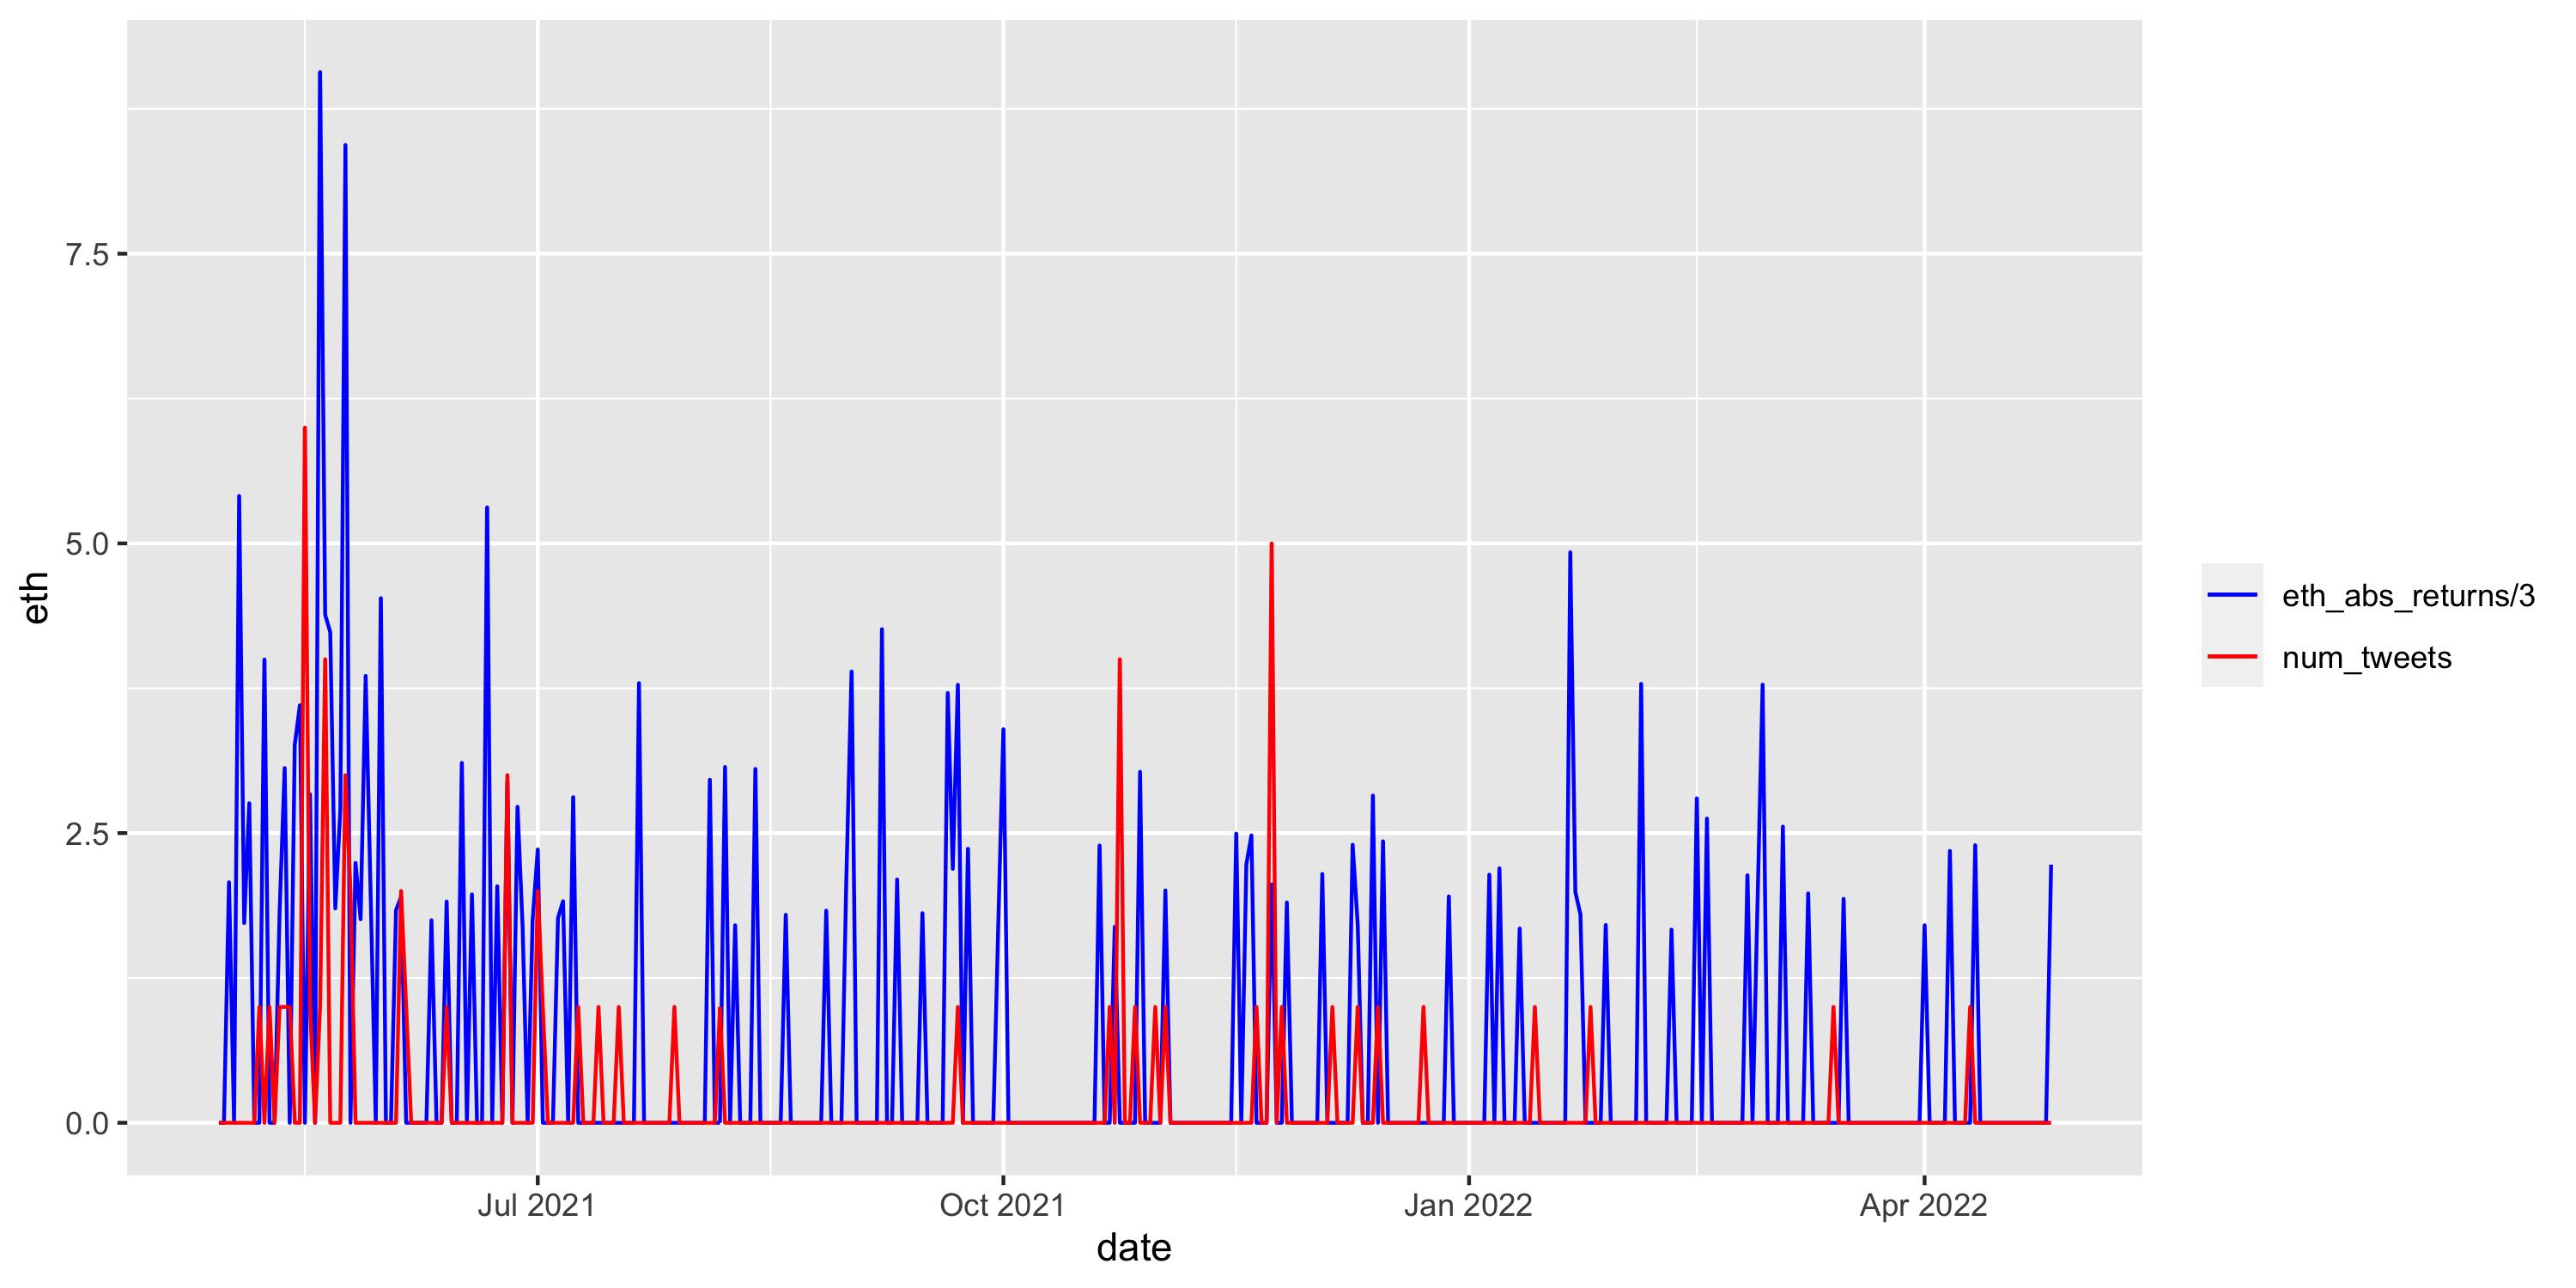
\includegraphics[width=16cm]{../figures/tweets_and_returns.png}
	\caption{The number of tweets and volatility of Ethereum. Ethereum volatility index in this figure was defined as its absolute return divided by 3. }
	\label{fig: tweets_and_returns}
\end{figure}

\subsection{Cryptocurrency Price on Yahoo Fiance}
Another major data source that we use in this project is the cryptocurrency price from Yahoo Finance. All major crypto prices for each day can be easily obtained in R by using the code under the ‘tidyquant’ package, such as tq\_get(), and we made some manipulations on the dataset based on our statistical and modeling needs. For instance, since the predictors and outcome variables in this project are daily returns, calculate by $$\frac{(\text{new adjusted closing price} - \text{old adjusted closing price})}{\text{old adjusted closing price} }*100,$$ we build our own function to help us do this. We also include some descriptions for the Cleaning/compilation/ manipulation process in R via comments. The raw dataset for the crypto prices will look something like the table \ref{Crypto prices} below.

\begin{table}[ht]
\centering
\begin{tabular}{rllllllll}
  \hline
 & symbol & date & open & high & low & close & volume & adjusted \\ 
  \hline
1 & ETH-USD & 2022-04-21 & 3077.83 & 3173.45 & 2962.41 & 2987.48 & 20783591093.00 & 2987.48 \\ 
  2 & ETH-USD & 2022-04-22 & 2986.94 & 3024.85 & 2942.36 & 2964.84 & 16782795477.00 & 2964.84 \\ 
  3 & ETH-USD & 2022-04-23 & 2964.80 & 2975.32 & 2926.74 & 2938.11 & 9116955609.00 & 2938.11 \\ 
  4 & ETH-USD & 2022-04-24 & 2937.35 & 2961.88 & 2922.13 & 2922.73 & 9696829579.00 & 2922.73 \\ 
  5 & ETH-USD & 2022-04-25 & 2922.99 & 3018.42 & 2804.51 & 3009.39 & 22332690614.00 & 3009.39 \\ 
  6 & ETH-USD & 2022-04-26 & 3008.95 & 3026.42 & 2786.25 & 2808.30 & 19052045399.00 & 2808.30 \\ 
   \hline
\end{tabular}
\caption{Crypto prices} 
\label{Crypto prices}
\end{table}

\section{Modeling and Analysis}
In many financial and business fields, the rationale of time series usually plays a critical role in terms of analyzing and predicting cryptocurrency data, such as stock returns. The reason is that the stock price data are taken sequentially in time, and each day’s stock price is highly correlated with the prices on other days. Meanwhile, it also have a correlation with other cryptocurrency prices. Hence, we can’t assume the error are independent. In addition, we usually do not consider its outcome as binary. Based on this idea, we divided our statistical models into two parts. The first part is using simple generalized linear model, such as logistic regression, whereas the second part is using more complex time series models, such as ARIMA, Bayesian structural time series (BSTS), and random forest.\\

\subsection{Model 1: Simple Logistic Regression Model}
A logistic regression model is a very common statistical model to predict a binary outcome, such as True/False, and Yes/No. It simply takes all the input values and outputs the probability of the outcome being True. The mathematics behind the logistical regression model can be interpreted as
$$P(Y_i=1)=logit^{-1}(X_i\bm{\beta})=\frac{e^{X_i\bm{\beta}}}{1+e^{X_i\bm{\beta}}},$$

\noindent where $X_i\bm{\beta}$ refers to the linear predictors.\\

\noindent In this logistic regression model, we first choose the adjusted daily returns for Ethereum as our outcome variables, set 1 if it is greater or equal to 5\%, 0 otherwise. Then, we replace the daily returns for doge, sol, and BTC with 1 if their return values are greater or equal to 5\%, 0 otherwise. These are the predictors. Finally, we add the number of tweets Elon musk posted on that day as another covariate, then fit a logistic regression model by applying the function glm(eth ~ doge + btc + sol + bch + num\_tweets, data = eth, family = 'binomial'), and make a further prediction on the returns for Ethereum itself.\\

\noindent The AUC score we obtained from this logistic regression model fit and prediction is close to 0.84 which means that most of the time, our model will be able to distinguish the positive class values from the negative class values. However, most of the time, stakeholders do not really care about whether the return is above or below a certain threshold, or does your model has a high AUC score. They may only focus on the amount of change for that day compared to the day before, and a simple logistic model might not be very useful in those cases, although it is a good model. Hence, we want to introduce other time series machine learning methods, which will be discussed in the rest of the paper. \\

\subsection{Model 2: Autoregressive Integrated Moving Average (ARIMA)}
Time series analysis is commonly used to forecast stock markets, and ARIMA is a classical approach to model stock prices. ARIMA models show more robust and efficient performance in short-term financial time series prediction than even the most popular ANNs techniques (Adebiyi et al., 2014). The price of cryptocurrencies is time series data. It is autocorrelated and the errors are not independent. Therefore, linear regression is not suitable for this case. Instead, ARIMA assumes correlation of errors and consists of two main components, AR (autoregressive) and MA (moving average). The AR model is where the output variable depends linearly on its previous values, while the MA model is where the outcome variable is determined by a linear combination of current and past white noise. I stands for integrated, which is achieved by differencing the data to make it stationary. Since we didn’t observe a clear trend in Ethereum returns, the integrated part was set to be 0. We defined the time lag p as 3 and the order of q as 3.\\

\noindent The $AR(p)$ model is defined as $$Y_t=c+\sum_{i=1}^{p}Y_{t-i}+\varepsilon_t.$$

\noindent The $MA(q)$ is defined as $$Y_t=\mu+\sum_{i=1}^{q}\theta_i\varepsilon_{t-i}+\varepsilon_t.$$
Independent variables, including several major cryptocurrencies, several stocks and bonds in the S\&P 500, some large technology stocks, etc., are also included in the ARIMA model. The mean squared error of the ARMIA model is 4.8.\\

\begin{figure}[H]
	\centering
	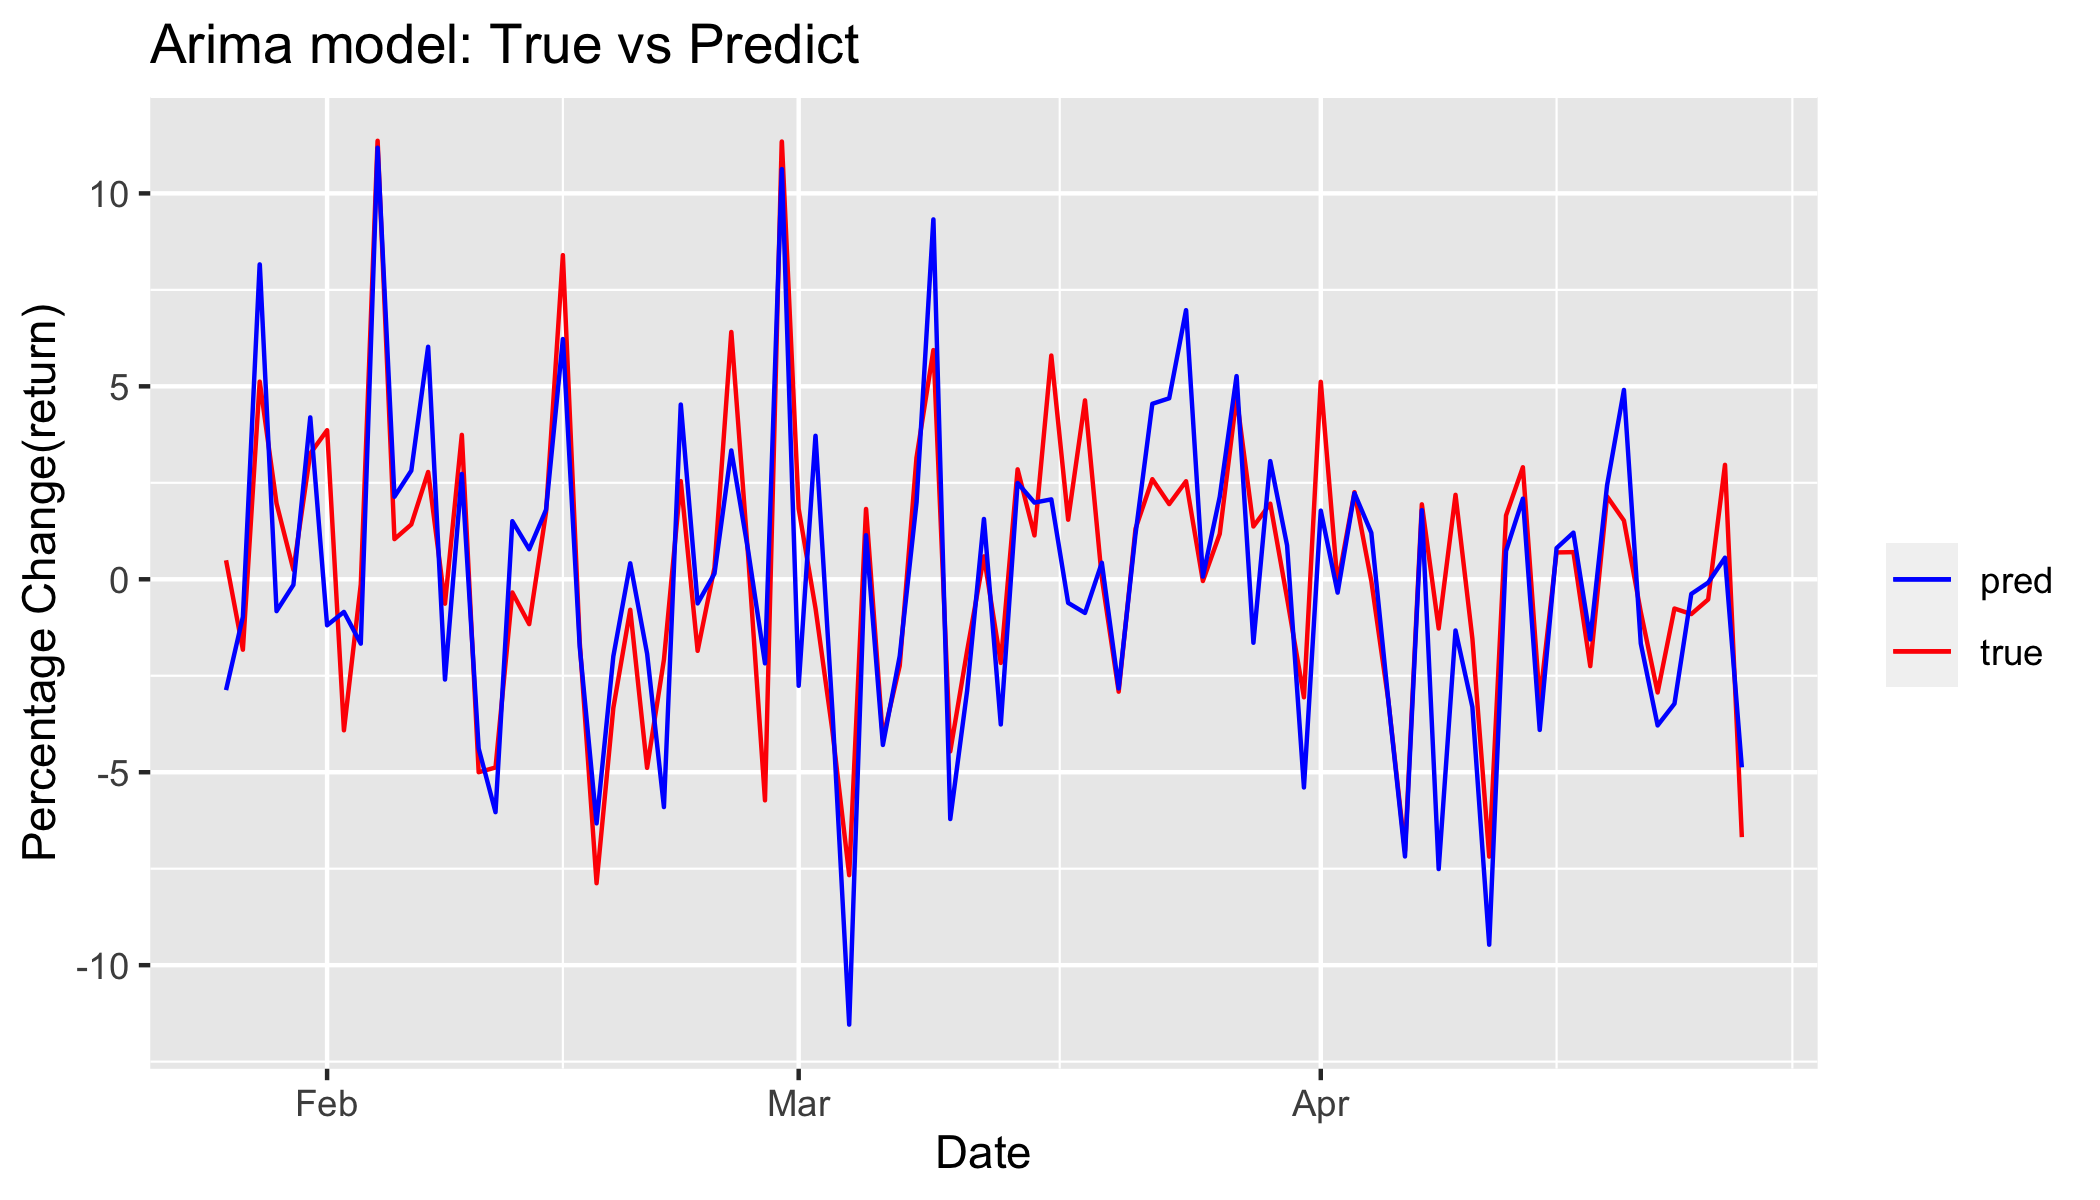
\includegraphics[width=16cm]{../figures/arima_true_and_predict.png}
	\caption{Model performance of Arima model (actual return vs predicted return)}
	\label{fig: arima_true_and_predict}
\end{figure}

\subsection{Model 3: Bayesian Structural Time Series (BSTS)}

\noindent Bayesian structural time series is a Bayesian version of ARIMA, which combines a structural time series and a regression model. BSTS has been shown to perform well in short-term forecasting and has been successfully used to capture trends between Google search trends and economics time series (Steven et al., 2013). Three main components are involved in BSTS model. First, the different state variables will be decomposed into time series by using a Kalman filter. Second, a spike-and-slab prior is used to select important regression predictors. Third, Bayesian model averaging method is used to smooth the predictors for a large number of models. As a by-product of Bayesian method, BSTS also provides the probability of each estimate of predictors.\\

\noindent We set the number of lags in $AR(p)$ model as 3 to specify the state component. Then, the set of independent variables that was used in the ARIMA model was also used for BSTS. The mean squared error for BSTS was 1.917, which was the best performance among all three models. Figure \ref{fig: bsts_true_and_predict} below shows the the predicted values are quite similar to the true values.

\begin{figure}[H]
	\centering
	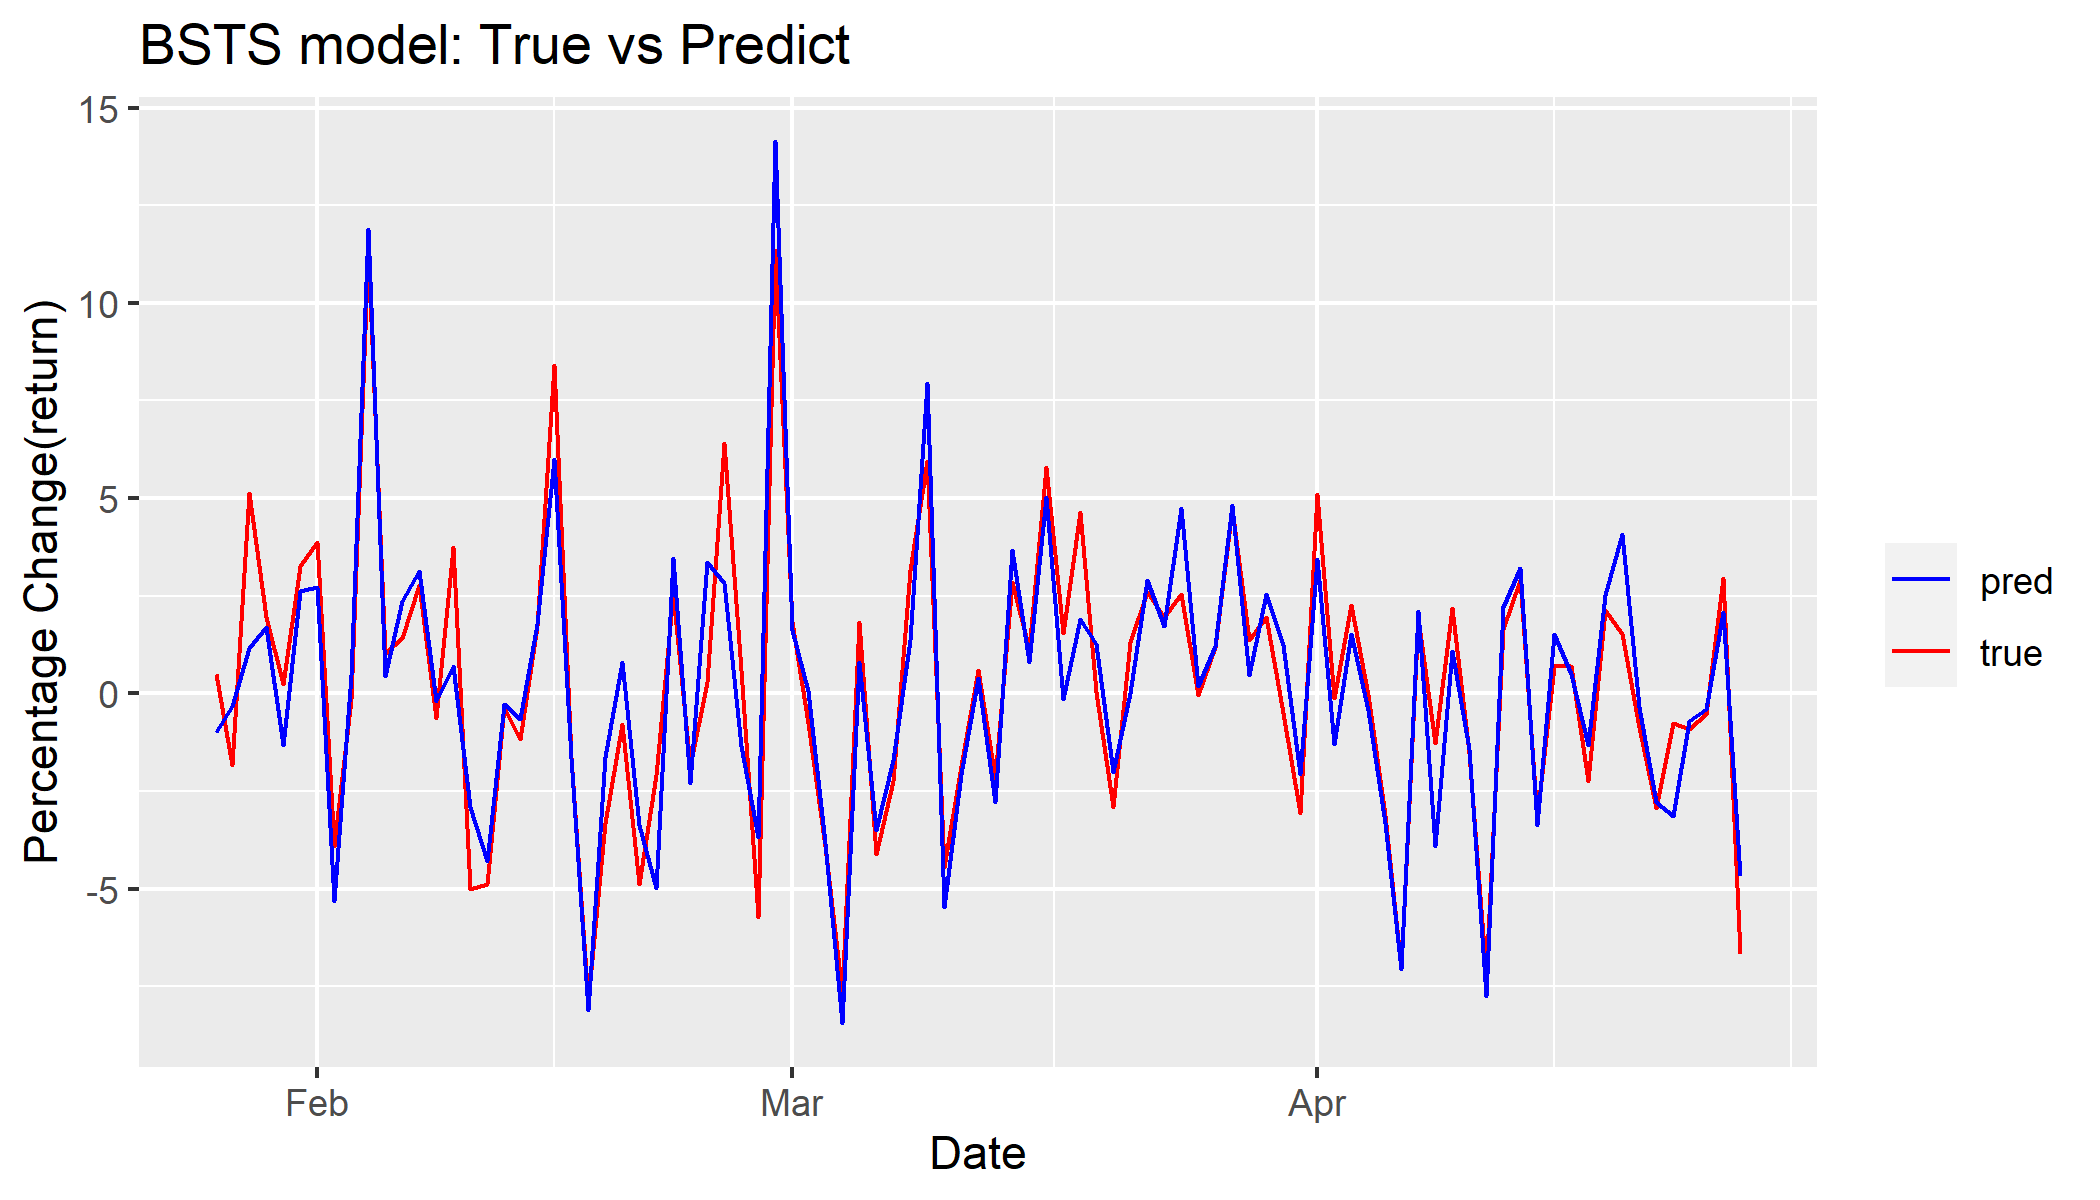
\includegraphics[width=16cm]{../figures/bsts_true_and_predict.png}
	\caption{model performance of BSTS model(actual return vs predicted return)}
	\label{fig: bsts_true_and_predict}
\end{figure}

\subsection{Model 3: Random Forest}

\noindent Before we talk about random forest, we need to introduce the idea of the decision tree since the random forest is basically a cluster or bag of decision trees. The fundamental rationale behind the decision tree is that for all training observations (predictors), we apply some criteria to each of them and find the best split values. Then, we apply Bagg, which refers to the  Bootstrap Aggregation (sampling with replacement), to our dataset as many as we want, fit a decision tree on each one, and combine their result. \\

\noindent In this random forest model for the cryptocurrency dataset, we intend to predict the return (change in percentage) for Ethereum on each day from 2022-01-26 to 2022-03-26 using the returns with other cryptocurrencies on the same day, such as DOGE, USDT, SOL, etc. For each data point in the backtest set, a random forest model with default numbers of trees is trained on the previous N points and predicts the next day’s return. The training set is built based on 90 days prior to the day that we want to predict. For instance, if we wish to predict the return for Ethereum in 2022-01-26, we need a training set from 2021-10-27 to 2022-01-25. After we finish the training process, we obtain the prediction for the return on each day and compare it to its true value. We also calculate the residual to see how well the fit is.\\

\noindent Figure \ref{fig: rf1_true_and_predict} is the predicted return value (blue) versus the actual return value(red). The x-axis is the Date and the y-axis is the change in percentage(return). As we can see, this random forest model isn't doing well in predicting the true values of return, and it even predicts the opposite direction on some days. Meanwhile, the calculated square of residual for this random forest model is about 7.47, which also supports that the performance of this model is quite bad compared to the ARIMA and BSTS. 

\begin{figure}[H]
	\centering
	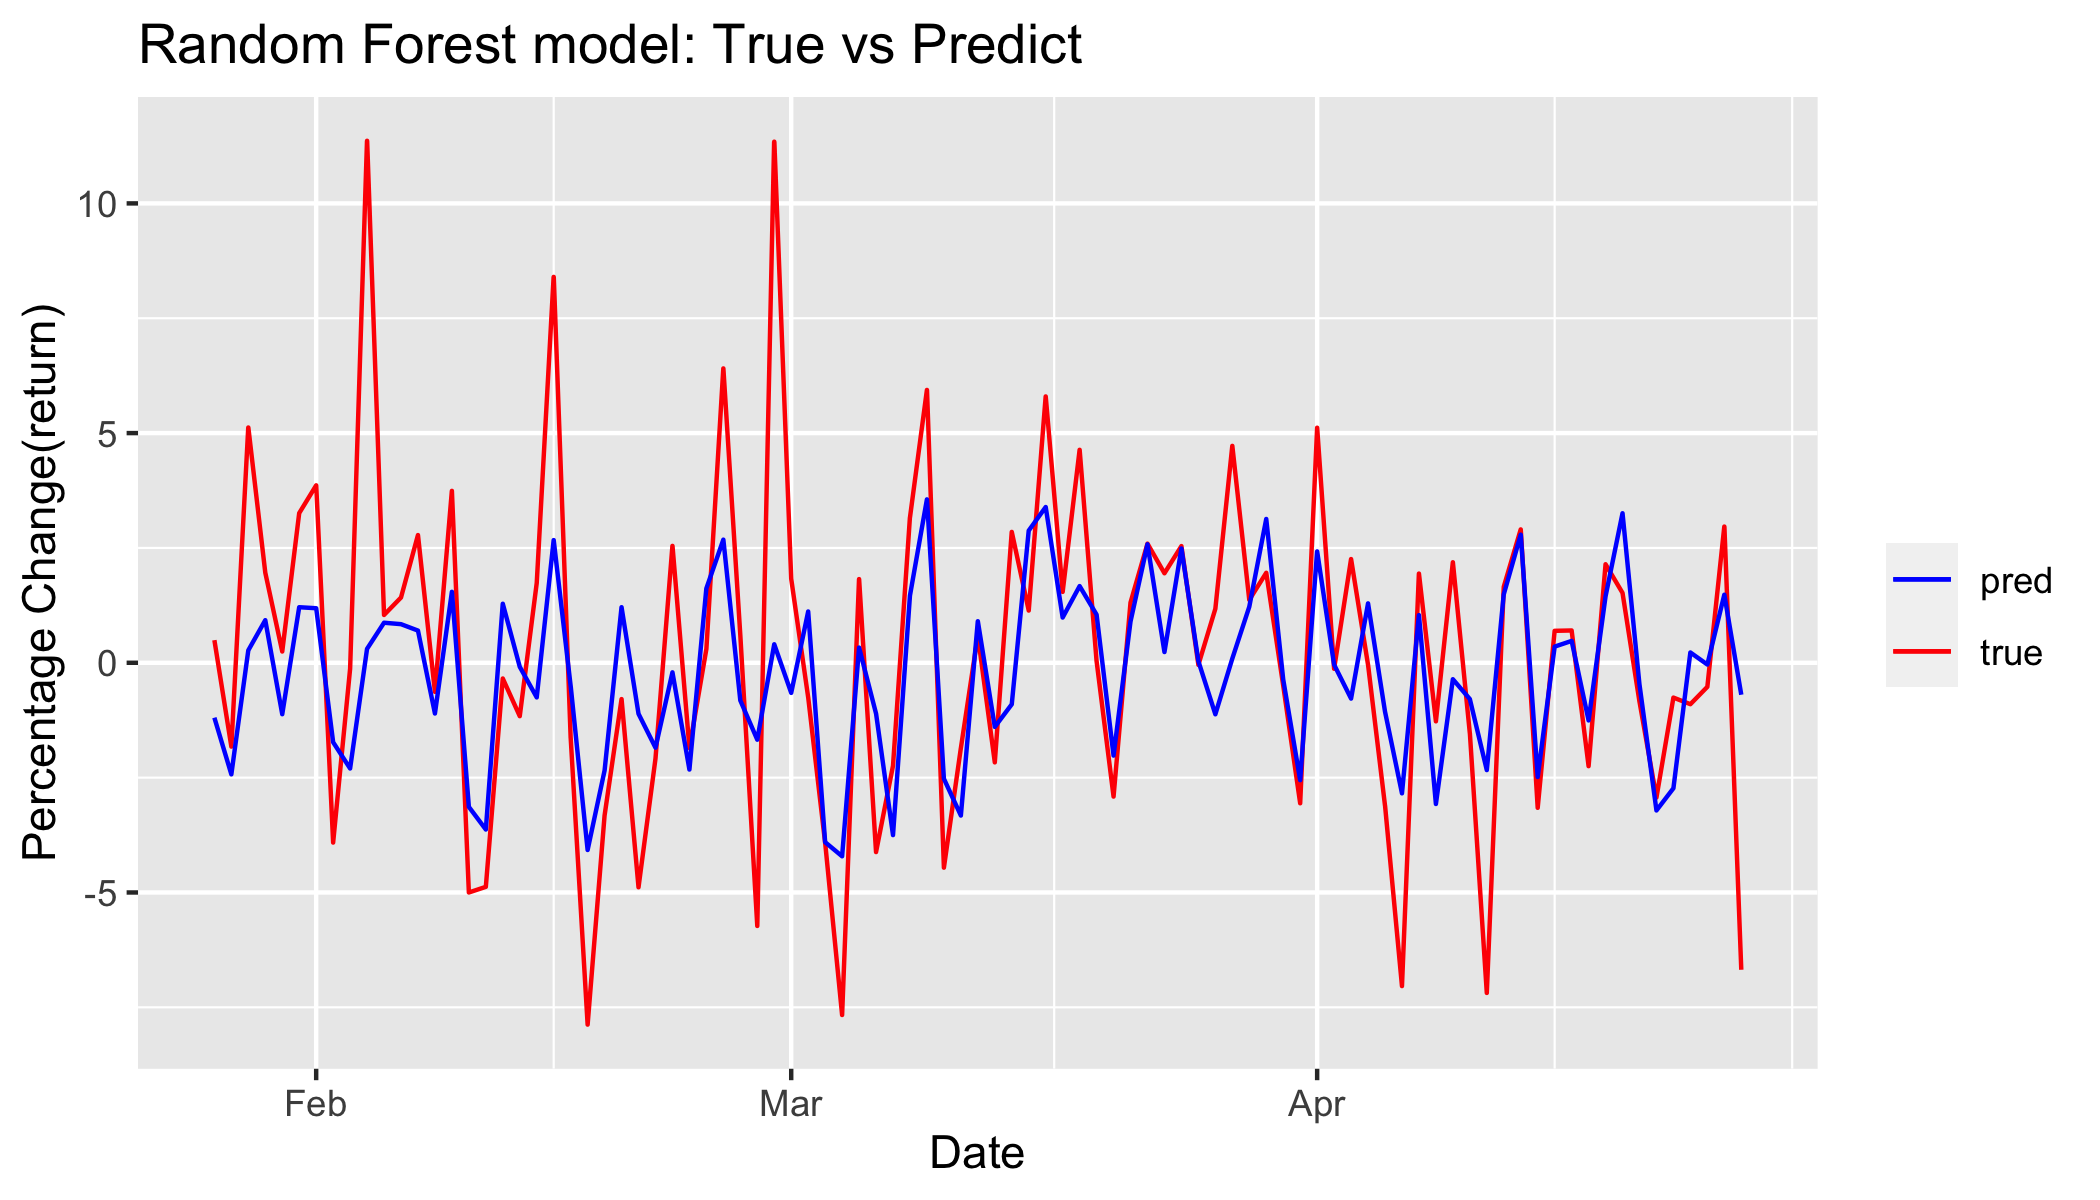
\includegraphics[width=16cm]{../figures/rf1_true_and_predict.png}
	\caption{model performance of BSTS model(actual return vs predicted return)}
	\label{fig: rf1_true_and_predict}
\end{figure}

\section{Conclusion and Call to Action}

By comparing the four machine learning models that we build above, we can clearly see that our prediction for cryptocurrency becomes more well performed in analyzing financial data after we introduce time series in our models. A traditional logistic regression model might not be able to give us a clear picture of how financial data changes day by day compared to the models with the time series, such as ARIMA and BSTS. On the other hand, those models with time series also perform differently in predicting the actual return value for each day. Based on the plots and square of residuals that we generated above, we can conclude that BSTS did the best job, although it still has some drawbacks. For instance, when we run the codes in R, BSTS toke the longest time, and sometimes the fitting function for BSTS  may not work very well on macOS. In short, we need to keep in mind that no one machine learning model can solve every problem in the real world, and different methods need to be adjusted based on the real situation we encounter. 

\section{Works Cited}

\noindent Ariyo, Adebiyi A., et al. “Stock Price Prediction Using the Arima Model.” 2014 UKSim-AMSS 16th International Conference on Computer Modelling and Simulation, 2014, https://doi.org/10.1109/uksim.2014.67.\\

\noindent Gareth James, Daniela Witten, Trevor Hastie, Robert Tibshirani. An Introduction to Statistical Learning : with Applications in R. New York :Springer, 2013.\\

\noindent Gelman, Andrew, et al. Regression and Other Stories. Cambridge University Press, 2020.\\

\noindent Larsen , Kim. “Sorry Arima, but I'm Going Bayesian.” Multithreaded, \\
\noindent https://multithreaded.stitchfix.com/blog/2016/04/21/forget-arima/.\\

\noindent Scott, Steven L., and Hal R. Varian. “Predicting the Present with Bayesian Structural Time Series.” SSRN, 1 Aug. 2013, https://papers.ssrn.com/sol3/papers.cfm?abstract\_id=2304426.

\end{document}